\section{Двухвыборочная задача}

Начнем с задачи с двумя выборками, описанной в предыдущей главе. Имеются выборки $\mathbf{z}$ и $\mathbf{y}$ из, возможно, различных распределений $F$ и $G$, и мы хотим проверить нулевую гипотезу $H_0: F = G$. Бутстреп проверка гипотез основана на тестовой статистике, как и проверка гипотез с помощью перестановочных тестов. В предыдущей главе тестовая статистика обозначалось как $\hat{\theta}$. Чтобы подчеркнуть, что тестовая статистика не обязательно должна быть оценкой параметра, обозначим ее здесь как $t(\mathbf{x})$. В примере с данными о мышах $t(\mathbf{x}) = \bar{z}-\bar{y}$, разница средних наблюдаемых значений $30.63$. Мы стремимся достигнуть уровень значимости
\begin{equation}\label{eq16.1}
    \text{ASL} = \mathrm{Prob}_{H_0}\left\{t(\mathbf{x}^{*}) \geq t(\mathbf{x})\right\}
\end{equation}
как в (15.4). Величина $t(\mathbf{x})$ фиксируется на своем наблюдаемом значении, а случайная величина $\mathbf{x}^{*}$ имеет распределение, заданное нулевой гипотезой $H_0$. Назовем это распределение $F_0$. Теперь вопрос состоит в том, что такое  $F_0$? В перестановочном тесте в предыдущей главе мы зафиксировали порядковую статистику $\mathbf{v}$ и определили $F_0$ как распределение возможных перестановок рангов $\mathbf{g}$. С другой стороны, бутсреп проверка гипотез использует оценку $F_0$, полученную методом подстановки. Обозначим объединенную выборку $\mathbf{x}$ и пусть ее эмпирическое распределение будет $\hat{F}_0$, полагая вероятность каждого элемента $\mathbf{x}$ равной $1/(n + m)$. Под $H_0$, $\hat{F}_0$ обеспечивает непараметрическую оценку общей популяции, которая порождает как $\mathbf{z}$, так и $\mathbf{y}$. Алгоритм 16.1 показывает, как вычисляется $\text{ASL}$.

\begin{center}
    \textit{Алгоритм 16.1}
\end{center}
\fbox{%
\parbox{\textwidth}{%
\begin{enumerate}
        \item Получить $B$ выборок размера $n + m$ с возвращением из $\mathbf{x}$. Обозначить первые $n$ наблюдений $\mathbf{z}^{*}$, а оставшиеся $m$ наблюдений $\mathbf{y}^{*}$.
        \item Оценить $t(\cdot)$ для каждой выборки,
        \begin{equation}\label{16.2}
            t(\mathbf{x}^{*b}) = \mathbf{\bar{z}}^{*}-\mathbf{\bar{y}}^{*}, \quad b = \ies{B}.
        \end{equation}
        \item Аппроксимировать $\text{ASL}_{\text{boot}}$ с помощью
        \begin{equation}\label{16.3}
            \widehat{\text{ASL}}_{\text{boot}} = \#\left\{t(\mathbf{x}^{*b}) \geq  t_{\text{obs}}\right\}/B,
        \end{equation}
        где $t_{\text{obs}} = t(\mathbf{x})$ наблюдаемое значение статистики.
    \end{enumerate}}%
}\\

Обратите внимание, что единственное различие между этим алгоритмом и перестановочным алгоритмом в уравнениях (15.17) и (15.18) состоит в том, что выборки осуществляются с возвращением, а не без него. Неудивительно, что он дает очень похожие результаты (левая часть рисунка 16.1). Была сгенерирована тысяча бутстреп выборок, и $120$ имели $t(\mathbf{x}^{*}) > 30.36$. Значение $\widehat{\text{ASL}}_{\text{boot}}$ составляет $120/1000 = 0.12$ в отличие от $0.152$ в перестановочном тесте.

\noindent
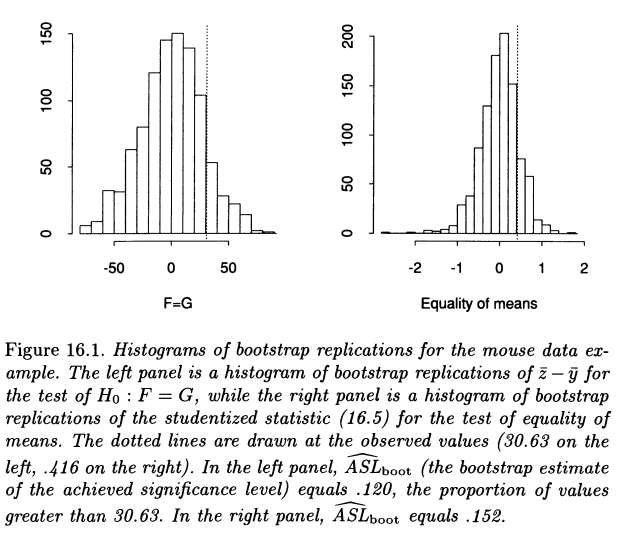
\includegraphics[width=\linewidth]{16/f16.1.png}

Более точный критерий можно получить за счет использования стьюдентизированной статистики. В приведенном выше тесте вместо $t(\mathbf{x}) = \bar{z}-\bar{y}$ мы могли бы использовать
\begin{equation}\label{eq16.4}
    t(\mathbf{x}) = \frac{\bar{z}-\bar{y}}{\bar{\sigma}\sqrt{1/n+1/m}},
\end{equation}
где $\bar{\sigma} = \left\{\left[\sum_{i=1}^{n}(z_i-\bar{z})^2 + \sum_{j=1}^{m}(y_j-\bar{y})^2\right]/\left[n+m-2\right]\right\}^{1/2}$. Это двухвыборочная статистика $t$, описанная в главе 15. Наблюдаемое значение $t(\mathbf{x})$ составило $1.12$. Повторение вышеупомянутого бутстреп алгоритма с использованием $t(\mathbf{x}^{*})$, определенной \ref{eq16.4}, привело к $134$ значениям из $1000$, превышающих $1.12$, и, следовательно, $\text{ASL}_{\text{boot}} = 0.134$. В этом вычислении мы использовали точно такой же набор бутстреп выборок, которые дали значение $0.12$ для $\widehat{\text{ASL}}_{\text{boot}}$ на основе $t(\mathbf{x}) = \bar{z}-\bar{y}$. В отличие от перестановочного теста, где мы показали, что стьюденизация не влияет на ответ, стьюденизация действительно приводит к другому значению $\widehat{\text{ASL}}_{\text{boot}}$. Однако в этом конкретном бутстреп подходе для задачи с двумя выборками разница обычно довольно мала.

Алгоритм 16.1 проверяет нулевую гипотезу о том, что две популяции идентичны, то есть $F = G$. Что, если бы мы хотели проверить только то, равны ли их средние значения? Один из подходов --- использовать двухвыборочную $t$-статистику \ref{eq16.4}. При нулевой гипотезе и в предположении нормально распределенных популяций с равными дисперсиями она имеет распределение Стьюдента с $n + m- 2$ степенями свободы. Она использует объединенную оценку стандартной ошибки $\bar{\sigma}$. Если мы не хотим предполагать, что дисперсии в двух популяциях равны, мы могли бы основывать тест на
\begin{equation}\label{eq16.5}
    t(\mathbf{x}) = \frac{\bar{z}-\bar{y}}{\sqrt{\hat{\sigma}^2_1/n + \hat{\sigma}^2_2/m}},
\end{equation}
где $\hat{\sigma}^2_1 = \sum_1^n(z_i-\hat{z})^2/(n-1)$, $\hat{\sigma}^2_2 = \sum_1^m(y_i-\hat{m})^2/(m-1)$. При генеральной совокупности имеющей нормальное распределение величина \ref{eq16.5} больше не имеет $t$-распределение Стьюдента, и поэтому был предложен ряд приближенных решений. В литературе это известно как проблема Беренса-Фишера. 

Предположение о равной дисперсии привлекательно для $t$-критерия, поскольку оно упрощает форму результирующего распределения. При рассмотрении бутрстреп теста для сравнения двух средних нет веских причин предполагать равные дисперсии, и, следовательно, мы не делаем этого предположения. Для продолжения нам потребуются оценки $F$ и $G$, в которых используется только предположение об общем среднем значении. Допустим, что $\bar{x}$ будет средним значением объединенной выборки, мы можем преобразовать обе выборки так, чтобы они имели среднее значение $\bar{x}$, а затем ресэмплировать каждую совокупность по отдельности. Процедура подробно описана в алгоритме 16.2. 

Результаты этого показаны на правой части рисунка 16.1. Значение $\widehat{\text{ASL}}_{\text{boot}}$ было $152/1000 = 0.152$.
\newpage
\begin{center}
    \textit{Алгоритм 16.2}
\end{center}
\fbox{%
\parbox{\textwidth}{%
\begin{center}
    \underline{Вычисление бутстреп статистики для проверки гипотезы равенстве средних}
\end{center}
\begin{enumerate}
        \item Пусть $\hat{F}$ задает одинаковую вероятность для точек $\widetilde{z}_i = z_i - \bar{z} + \bar{x}$, $i~=~\ies{n}$, а $\hat{G}$ задает одинаковую вероятность для точек $\widetilde{y}_i = y_i - \bar{y} + \bar{x}$, $i~=~\ies{m}$, где $\bar{z}$ и $\bar{y}$ --- групповое среднее, а $\bar{x}$ --- средние по объединенной выборке.
        \item Сформировать $B$ бутстреп выборок $(\mathbf{z}^{*},\,\mathbf{y}^{*})$, где $\mathbf{z}^{*}$ выборка с возвращением из $\widetilde{z}_1,\widetilde{z}_2,\ldots,\widetilde{z}_n$ и $\mathbf{y}^{*}$ выборка с возвращением из $\widetilde{y}_1,\widetilde{y}_2,\ldots,\widetilde{y}_m$.
        \item Вычислить $t(\cdot)$, определенное в \ref{eq16.5}, для каждой выборки
        \begin{equation}\label{eq16.6}
            t(\mathbf{x}^{*b}) = \frac{\bar{z}^{*}-\bar{y}^{*}}{\sqrt{\hat{\sigma}^{2*}_1/n + \hat{\sigma}^{2*}_2/m}}, \quad b = \ies{B}.
        \end{equation}
        \item Аппроксимировать $\text{ASL}_{\text{boot}}$ с помощью
        \begin{equation}\label{16.7}
            \widehat{\text{ASL}}_{\text{boot}} = \#\left\{t(\mathbf{x}^{*b}) \geq  t_{\text{obs}}\right\}/B,
        \end{equation}
        где $t_{\text{obs}} = t(\mathbf{x})$ наблюдаемое значение статистики.
    \end{enumerate}}%
}\\